\documentclass{report}
\usepackage[utf8]{inputenc}
\usepackage[T1]{fontenc}  
\usepackage[french]{babel}
\usepackage{fullpage}
\usepackage{graphicx}
\usepackage{caption}
\usepackage{subcaption}
%\usepackage{pst-all}
%\usepackage[toc,page]{appendix}
\usepackage[final]{pdfpages}
%\usepackage{lscape}
\usepackage{verbatim}
\title{Image 3D \\Estimation du bruit et débruitage}
\author{\textsc{hitier} Jérémy}
\date{\today}
\begin{document}
\maketitle
\tableofcontents
\newpage
\newpage

\chapter{TD1 - Estimation du bruit}
\section{Génération du bruit et estimation du PSNR}
\subsection{Génération du bruit gaussien}

On génère un bruit gaussien de 5\% sur l'image 3D MRIT1w. Ci-dessous les résultats obtenus.
\begin{figure}[h]
\centering
	\begin{subfigure}[b]{0.4\textwidth}
	\centering
	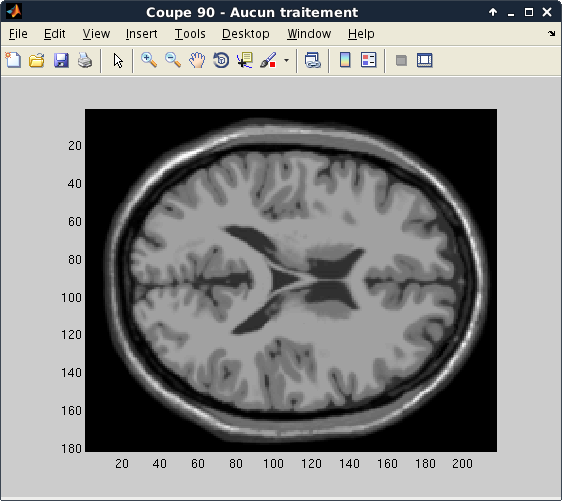
\includegraphics[width = 6cm]{coupe90.png}
	\caption{Original}
	\end{subfigure}
	~
	\begin{subfigure}[b]{0.4\textwidth}
	\centering
	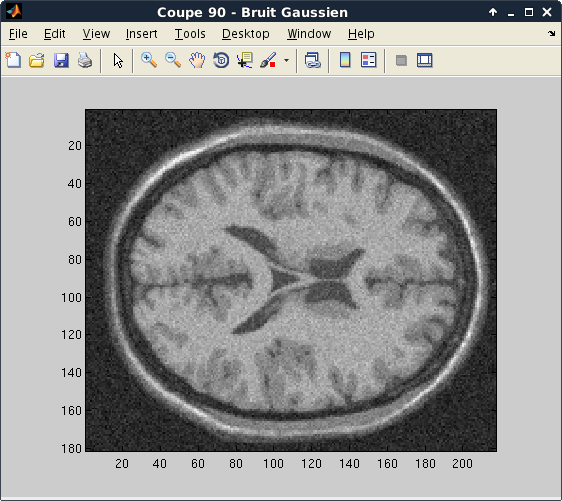
\includegraphics[width = 6cm]{coupe90Gauss.png}
	\caption{Avec 5\% de bruit gaussien}
	\end{subfigure}
	\caption{Visualisation de la 90ème coupe}
\end{figure}
\newpage
\subsection{Génération du bruit ricien}

On génère un bruit ricien de 5\%. Ci dessous le résultat (Fig. \ref{fig:ricien}):

\begin{figure}[ht!]
	\centering
	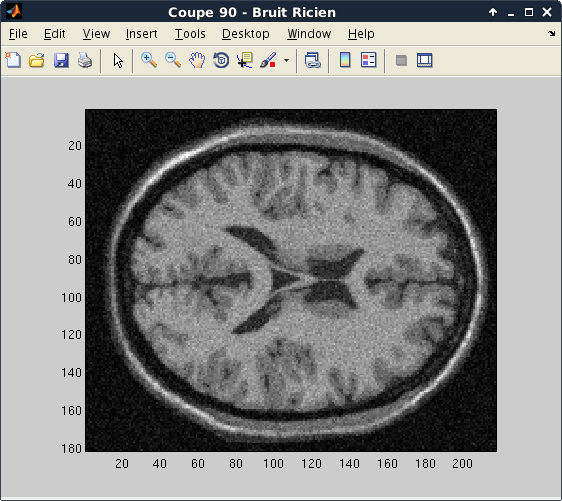
\includegraphics[width = 8cm]{coupe90Rici.png}
	\caption{\label{fig:ricien}Bruit Ricien à 5 sur la coupe 90\%}
	
\end{figure}

On calcul ensuite le PSNR pour des niveaux de bruit ricien allant de 1\% à 21\% tous les 1\%. Les résultats sont reportés dans le graphique suivant (Fig. \ref{fig:psnr}).
\begin{figure}[ht!]
	\centering
	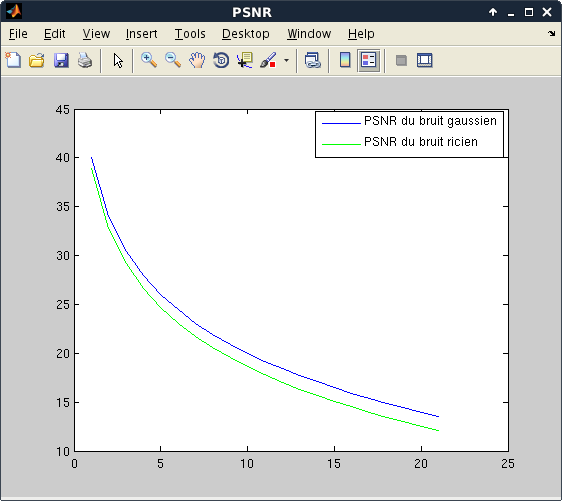
\includegraphics[width = 8cm]{PSNR.png}
	\caption{\label{fig:psnr}PSNR}
	
\end{figure}

\section{Estimation du niveau de bruit dans le cas gaussien à l'aide de l'estimateur MAD}
\subsection{La transfomée en ondelette}
La transformée en ondelette permet de passer notre image dans le domaine fréquentiel tout en conservant de l'information temporelle. Ci-dessous les coupes LLL et HHH:
\begin{figure}[h]
\centering
	\begin{subfigure}[h]{0.42\textwidth}
	\centering
	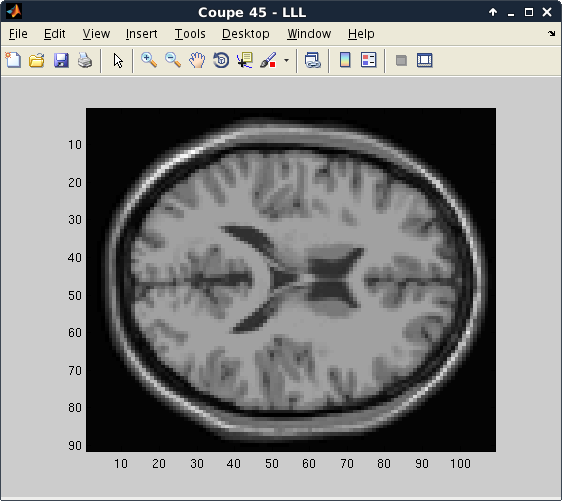
\includegraphics[width = 6cm]{coupe45LLL.png}
	\caption{Bande LLL}
	\end{subfigure}
	~	
	\begin{subfigure}[h]{0.42\textwidth}
	\centering
	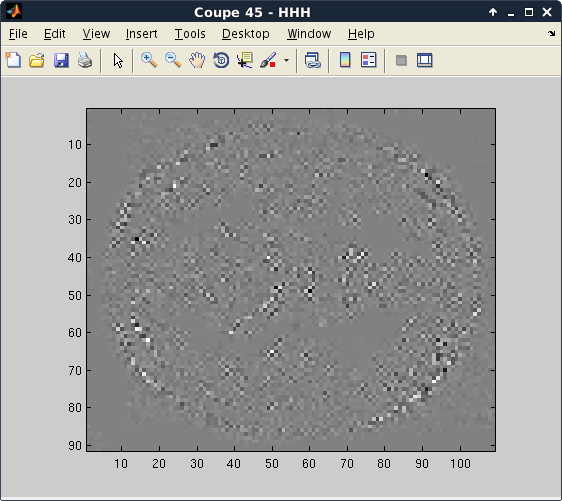
\includegraphics[width = 6cm]{coupe45HHH.png}
	\caption{Bande HHH}
	\end{subfigure}
	\caption{Visualisation des bandes LLL et HHH après transformée en ondelette}
\end{figure}

\subsection{L'estimateur MAD}
Afin d'estimer le niveau de bruit dans notre image, on utilise l'estimateur "Median Absolute Deviation".
L'erreur d'estimation a été calculé pour les niveaux de bruit gaussien de 1 à 21\% et les résultats sont ci-dessous:
\begin{figure}[!ht]
	\centering
	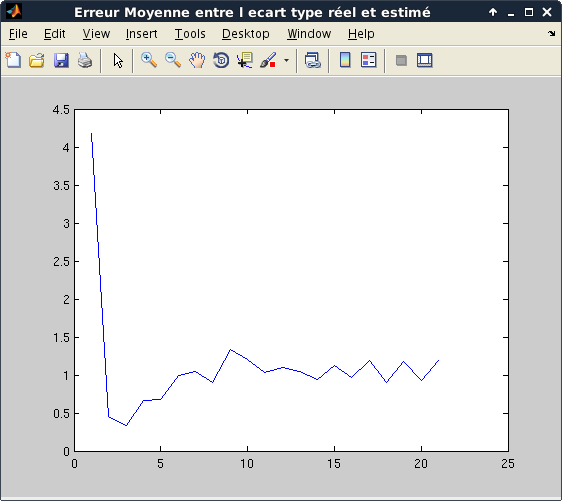
\includegraphics[width = 8cm]{erreurMAD.png}
	\caption{\label{fig:mad}Courbe d'erreur pour l'estimateur MAD}
	
\end{figure}
~\\On peut voir que l'erreur réduit fortement puis se stabilise.

\section{Estimation à l'aide de la distribution des statistiques locales de l'image}
\subsection{Les moyennes locales}
Résultat du filtre par moyennes locales (Fig. \ref{fig:lm}):
\begin{figure}[!ht]
	\centering
	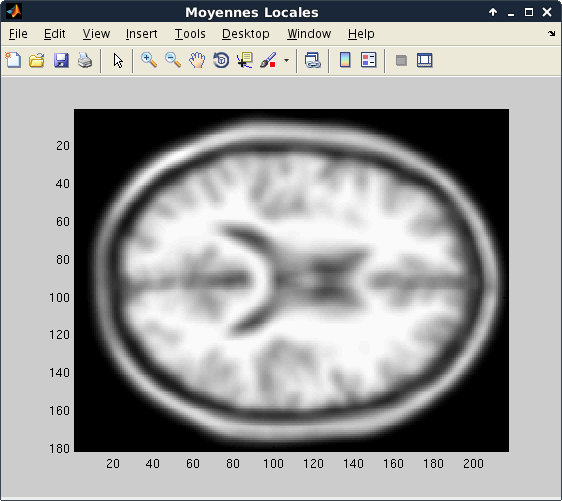
\includegraphics[width = 8cm]{moyenneLocal.png}
	\caption{\label{fig:lm}Image par filtre des moyennes locales}
\end{figure}

\subsection{Les variances locales}
Résultat du filtre par variances locales (Fig. \ref{fig:lv}):

\begin{figure}[!ht]
	\centering
	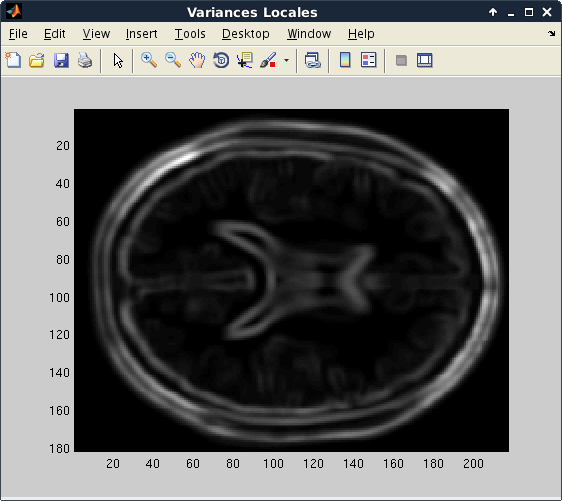
\includegraphics[width = 8cm]{varianceLocal.png}
	\caption{\label{fig:lv}Image par filtre des variances locales}
\end{figure}

\section{Comparaison}
\subsection{Moyennes locales contre Variances locales}
Le graphique suivant présente l'erreur d'estimation entre les deux estimateurs ci-dessus:
\begin{figure}[!ht]
	\centering
	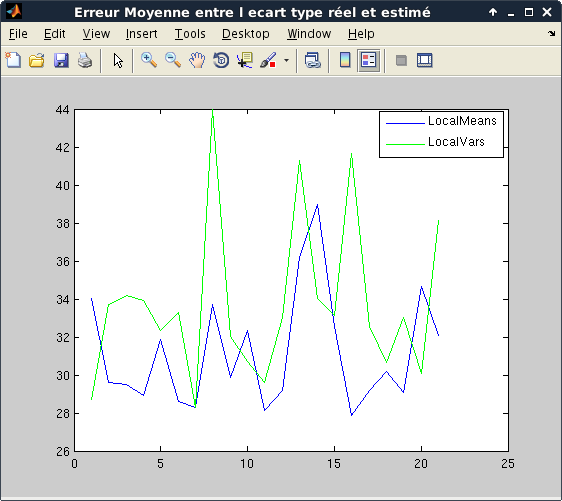
\includegraphics[width = 8cm]{erreurStat.png}
	\caption{\label{fig:errstat}Courbe d'erreur pour les estimateurs statistiques}
\end{figure}
~\\
L'estimateur utilisant les moyennes locales donne de meilleurs résultats que celui des variances locales.

\chapter{TD2 - Méthode de débruitage}
%\section{Filtre gaussien}
%La formule utile pour coder le filtre gaussien est celle d'une somme pondérée des observation bruitées :
%$$ \hat{x}(p) = \frac{1}{C_{p}}\sum_{q}y(q)w(p,q) $$
%Où $y(q)$ correspond à la valeur du voxel dans l'image bruitée.\\
%Les poids sont calculé grâce à la distance entre les voxels p et q de l'image:
%$$ w(p,q) = \exp(-\frac{||p-q||^2}{2\sigma_{s}^2}) $$
%Et enfin la formule de la constante de normalisation :
%$$ C_{p} = \sum_{q}w(p,q) $$
%
%Voir la section des Comparaisons pour les résultats. Des problèmes ont été rencontrés pour récupérer certaines informations lors des tests, notamment pour le calcul du PSNR qui se retrouvait négatif après le filtrage, la seul façon d'obtenir un PSNR positif a été d'inverser la comparaison, ce qui ne donne pas un résultat cohérent de mon point de vue. Un autre problème a été rencontré lors de l'extraction de l'image du bruit qui ne paraît pas cohérente non plus à la vue de celles obtenues pour le filtre bilatéral et pour le filtre par seuillage (voir figure 2.1 et 2.2).
%
%\section{Filtre par seuillage d'ondelette}
%Le filtrage par seuillage d'ondelette se fait ici sur l'utilisation du seuillage dur sur la sous-bande HHH de l'image qui contient les plus hautes fréquences de notre image.
%
%Le seuillage dur se défini comme un seuillage d'image traditionnel. Si la valeur absolue du coefficient est supérieur au seuil alors on garde la valeur, sinon on affecte 0.
%Dans notre cas, le seuil est calculé grâce à la formule suivante:
%$$ \lambda = \sigma\sqrt{2\log_{10}M} $$
%Où $M$ est la taille de la sous-bande.
%Voir la section des Comparaisons pour les résultats.
%
%\section{Filtre bilatéral}
%Le filtre bilatéral peut lui aussi être vu comme une somme pondérée des observation bruitées, seulement la fonction de calcul des poids subit une modification et s'appuie sur 2 noyaux désormais. Le premier est un noyau gaussien tandis que le second est calculé grâce à la distance entre les valeurs des voxels p et q dans l'image bruitée : 
%$$ w(p,q) = \exp(-\frac{||p-q||^2}{2\sigma_{s}^2})\exp(-\frac{||y(p)-y(q)||^2}{2\sigma_{i}^2})$$
%Voir la section des Comparaisons pour les résultats.
%
%\section{Filtre des moyennes non locales}
%Le filtre des moyennes non locales comme le filtre gaussien et bilatéral est une somme pondérée des observation bruitées, mais avec un noyaux différent. Celui-ci se base sur la distance des valeurs des voxels voisin à p et à q dans l'image bruitée :
%
%$$ w(p,q) = \exp(-\frac{||y(N_{p})-y(N_{q})||^2}{2\sigma_{i}^2})$$
%
%Malheureusement, par manque de temps, ce filtre n'a pas été implémenté, il n'apparaîtra donc pas dans les tests de comparaison.
%
%\section{Comparaison}
%Comme on peut le voir dans le tableau de résultat (figure 2.1) si on s'attache aux valeurs du PSNR c'est le filtrage par seuillage d'ondelette qui nous retourne l'image la plus fidèle à l'image de départ, cependant le PSNR ne reflète pas la qualité visuelle de celle-ci.
%
% En effet, si l'on regarde la comparaison des résultats sur la 90ème coupe, on peut voir que même si le seuillage d'ondelette nous rend un résultat plus que correct, il a tendance à rendre un image encore floue et pas totalement débruitée. Le filtrage gaussien lui nous retourne une image bien débruitée mais beaucoup trop floue tandis que le filtre bilatéral nous renvoi une image bien débruitée, pas floue, mais efface certain détail.
%
%
%\begin{figure}[h]
%\begin{tabular}{|c|c|c|c|c|}
%\hline 
%Image & Image Bruité à 7\% & Filtre gaussien s=0.25 & Filtre gaussien s=0.5 & Filtre gaussien s=0.75 \\ 
%\hline 
%PSNR & 23.0974 & 14.1695 & 13.9072 & 12.5571 \\ 
%\hline 
%Image & Filtre gaussien s=1 & Filtre gaussien s=1.25 & Filtre gaussien s=1.5 & Filtre gaussien s=1.75\\
%\hline
%PSNR & 11.6445 & 11.1876 & 10.9691 & 10.8622 \\
%\hline
%Image & Filtre gaussien s=2 & Filtre par seuillage & Filtre bilatéral & • \\ 
%\hline 
%PSNR  & 10.8058 & 30.1410 & 27.3401 & • \\ 
%\hline 
%\end{tabular} 
%\caption{Tableau de comparaison du PSNR entre les différents filtres}
%\end{figure}
%
%
%\begin{figure}[h]
%\centering
%	\begin{subfigure}[t]{0.4\textwidth}
%	\centering
%	\includegraphics[scale=0.35]{Original.png}
%	\caption{Original}
%	\end{subfigure}
%	~
%	\begin{subfigure}[t]{0.4\textwidth}
%	\centering
%	\includegraphics[scale=0.35]{Gauss-7p.png}
%	\caption{Image bruité avec 7\% de bruit gausien}
%	\end{subfigure}
%	
%	\begin{subfigure}[b]{0.42\textwidth}
%	\centering
%	\includegraphics[scale=0.35]{GaussDenoise-k7-s2.png}
%	\caption{filtre avec un noyau de 7 et un sigma de 2}
%	\end{subfigure}
%	~	
%	\begin{subfigure}[b]{0.42\textwidth}
%	\centering
%	\includegraphics[scale=0.35]{BruitGauss.png}
%	\caption{Image du bruit retiré par le filtre gaussien}
%	\end{subfigure}
%
%	\begin{subfigure}[b]{0.42\textwidth}
%	\centering
%	\includegraphics[scale=0.35]{WaveletDenoise.png}
%	\caption{filtre par seuillage d'ondelette}
%	\end{subfigure}
%	~	
%	\begin{subfigure}[b]{0.42\textwidth}
%	\centering
%	\includegraphics[scale=0.35]{BruitWavelet.png}
%	\caption{Image du bruit retiré par le seuillage d'ondelette}
%	\end{subfigure}
%	
%	\begin{subfigure}[b]{0.42\textwidth}
%	\centering
%	\includegraphics[scale=0.35]{BilateralDenoise-k5-s40.png}
%	\caption{filtre bilatéral avec un noyau de 5 et les 2 sigmas à 40}
%	\end{subfigure}
%	~	
%	\begin{subfigure}[b]{0.42\textwidth}
%	\centering
%	\includegraphics[scale=0.35]{BruitBilateral.png}
%	\caption{Image du bruit retiré par le filtre bilatéral}
%	\end{subfigure}
%	\caption{Visualisation de la 90ème coupe}
%\end{figure}
%%inserer les résultats.

\end{document}
